\documentclass[a4paper,12pt]{article}

\usepackage[T2A]{fontenc}
\usepackage[english,russian]{babel}
\usepackage[utf8]{inputenc}
\usepackage{listings}
%\usepackage{pscyr}
\usepackage{graphicx}
%\usepackage{amstext}
%\usepackage{amssymb}
%\usepackage{lscape}
\usepackage{verbatim}
% \newcommand{\No}{\textnumero}


% \PassOptionsToPackage{unicode=true}{hyperref} % options for packages loaded elsewhere
% \PassOptionsToPackage{hyphens}{url}
% % use upquote if available, for straight quotes in verbatim environments
% \IfFileExists{upquote.sty}{\usepackage{upquote}}{}
% % use microtype if available
% \IfFileExists{microtype.sty}{%
% \usepackage[]{microtype}
% \UseMicrotypeSet[protrusion]{basicmath} % disable protrusion for tt fonts
% }{}
% \IfFileExists{parskip.sty}{%
% \usepackage{parskip}
% }{% else
% \setlength{\parindent}{0pt}
% \setlength{\parskip}{6pt plus 2pt minus 1pt}
% }


% PDF search & cut'n'paste
\usepackage{cmap}
\usepackage{listings}
\usepackage{url}
\usepackage{color}
\usepackage{textcomp}
\usepackage[colorlinks]{hyperref}
\hypersetup{
            pdfborder={0 0 0},
            breaklinks=true}
\urlstyle{same}  % don't use monospace font for urls
\usepackage{longtable,booktabs}

\lstset{
	language=C,
	tabsize=4,
	breaklines=true,
	basicstyle=\footnotesize,
	identifierstyle=\ttfamily,
	extendedchars=true,
}


\lstnewenvironment{cpp_code}[1][]{
    \lstset{
        language=C++,
        numbers=left,
        stepnumber=1,
        breaklines=true,
        basicstyle=\linespread{1.0}\ttfamily,
        keywordstyle=\color{blue}\ttfamily,
        stringstyle=\color{red}\ttfamily,
        commentstyle=\color{OliveGreen}\ttfamily,
        morecomment=[l][\color{magenta}]{\#}
        columns=fullflexible,
        postbreak=\mbox{\textcolor{red}{$\hookrightarrow$}\space},
        escapeinside={(*@}{@*)},
        showstringspaces=false
    }
    \lstdefinestyle{nonumbers}
    {numbers=none}
}{}

    
\lstnewenvironment{py_code}[1][]{
    \lstset{
        language=python,
        stepnumber=1,
        breaklines=true,
        basicstyle=\linespread{1.0}\ttfamily,
        keywordstyle=\color{blue}\ttfamily,
        stringstyle=\color{red}\ttfamily,
        commentstyle=\color{OliveGreen}\ttfamily,
        morecomment=[l][\color{magenta}]{\#}
        columns=fullflexible,
        otherkeywords={self},
        postbreak=\mbox{\textcolor{red}{$\hookrightarrow$}\space},
        escapeinside={(*@}{@*)},
        showstringspaces=false,
    }
    \lstdefinestyle{nonumbers}
    {numbers=none}
}{}

\lstnewenvironment{code}[1][]{
    \lstset{
        language=bash,
        breaklines=true,
        basicstyle=\linespread{1.0}\ttfamily,
        keywordstyle=\color{blue}\ttfamily,
        stringstyle=\color{red}\ttfamily,
        commentstyle=\color{OliveGreen}\ttfamily,
        morecomment=[l][\color{magenta}]{\#}
        columns=fullflexible,
        postbreak=\mbox{\textcolor{red}{$\hookrightarrow$}\space},
        escapeinside={(*@}{@*)},
    }
    \lstdefinestyle{nonumbers}
    {numbers=none}
}{}

\lstset{
    language=python,
    breaklines=true,
    basicstyle=\linespread{1.0}\ttfamily,
    keywordstyle=\color{blue}\ttfamily,
    stringstyle=\color{red}\ttfamily,
    commentstyle=\color{olivegreen}\ttfamily,
    morecomment=[l][\color{magenta}]{\#}
    columns=fullflexible,
    postbreak=\mbox{\textcolor{red}{$\hookrightarrow$}\space},
    escapeinside={(*@}{@*)},
}

\makeatletter
\renewcommand\paragraph{\@startsection{paragraph}{4}{\z@}%
            {-2.5ex\@plus -1ex \@minus -.25ex}%
            {1.25ex \@plus .25ex}%
            {\normalfont\normalsize\bfseries}}
\makeatother

\setcounter{secnumdepth}{3} % how many sectioning levels to assign numbers to
\setcounter{tocdepth}{4}    % how many sectioning levels to show in ToC
\renewcommand{\rmdefault}{ftm}
% \renewcommand{Оглавление}
\linespread{1.3} %1.5 межстрочный интервал
\usepackage[left=3cm,right=2.5cm,top=3cm,bottom=3cm,bindingoffset=0cm]{geometry}



\begin{document}


% \begin{titlepage}
	\begin{center}
	\textsc{\normalsize{ФЕДЕРАЛЬНОЕ ГОСУДАРСТВЕННОЕ АВТОНОМНОЕ ОБРАЗОВАТЕЛЬНОЕ}}\\
\textsc{\normalsize{УЧРЕЖДЕНИЕ ВЫСШЕГО ОБРАЗОВАНИЯ}}\\
\textsc{\normalsize{НАЦИОНАЛЬНЫЙ ИССЛЕДОВАТЕЛЬСКИЙ УНИВЕРСИТЕТ}}\\
\textsc{\normalsize{{«ВЫСШАЯ ШКОЛА ЭКОНОМИКИ»}}\\
	\normalsize{ФАКУЛЬТЕТ КОМПЬЮТЕРНЫХ НАУК}}
	\\[.5cm]
	\normalsize{\underline{Дьячков Леонид Андреевич}}\\[.5cm]

	\normalsize{МАГИСТЕРСКАЯ ДИССЕРТАЦИЯ}\\[.8cm]

	{\normalsize {\ul{\textbf{Исследование и разработка методов динамического анализа для определения входных данных влияющих на выполнение условных переходов}}}} \\[.3cm]
	{\normalsize {\ul{\textbf{Research and Development of Methods of Dynamic Analysis for Detecting Input Data Affecting Condition Branches Execution}}}}\\[.5cm]

	по направлению подготовки \underline{09.04.04 Программная инженерия}\\
	образовательная программа \underline{«Системное программирование»}

	\begin{flushleft}
	Cтудент\\
	\underline{\hspace{3cm}}\\
	Л.А. Дьячков\\
	\end{flushleft}
	\begin{flushright}
		
		Научный руководитель: \\ 
		д.ф.-м.н, проф. \\
		\underline{\hspace{3cm}}\\
		А.К. Петренко \\
		\\
		Соруководитель: \\ 
		к.ф.-м.н, с.н.с ИСП РАН \\
		\underline{\hspace{3cm}}\\
		Ш.Ф. Kурмангалеев \\
	\end{flushright}
	\vfill
	
	Москва, 2019
	\end{center}

\end{titlepage}

\tableofcontents
\chapter{Введение}


В последние годны наблюдается заметный рост количества уязвимостей в программном обеспечении. Так, согласно статистике \cite{CVEstats}, в $2016$ году было обнаружено $6447$ уязвимостей, в $2017$ --  $14714$, a в $2018$ -- $16555$. Это связано как с объемом и сложностью, разрабатываемого программного обеспечения, так и с развитием техник тестирования безопасности.

\begin{figure}[h]
    \center{
        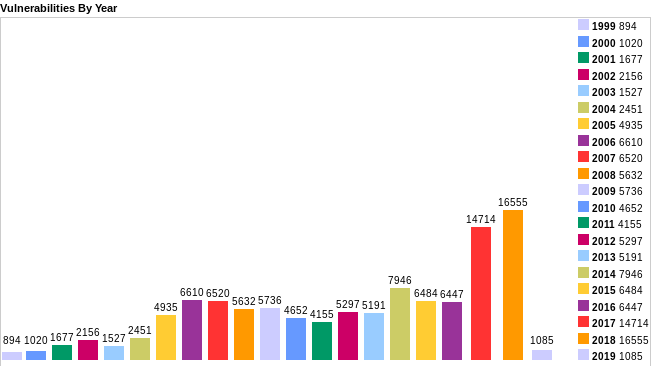
\includegraphics[scale=0.5]{img/cve_stats.png}
    }
    \caption{Cтатистика опубликованных уязвимостей за последние 20 лет}
    \label{fig:image}
\end{figure}

Одним из популярных подходов к автоматизации поиска уязвимостей является фаззинг-тестирование. Это
техника тестирования программного обеспечения, заключающая в передаче приложению на вход неправильных, неожиданных или случайных данных.

P

Фаззинг-тестирование является достаточно популярным подходом в тестировании на безопасность.


В последние годы наблюдается рост интереса к фаззинг-тестированию.



\chapter{Обзор}

% \chapter{Методы реализации динамического анализа}

\section{Динамический Анализ}

Динамический анализ - это анализ, заключающийся в непосредственном выполнении кода. Однако, просто запустить программу может быть недостаточно. Существует несколько способов получения дополнительной информации во время выполнения:

\begin{itemize}
\item {\em Исполнение кода в виртуальном окружении}. При данном подходе программа запускается внутри некоторого программного эмулятора. Например qemu \cite{QEMU}.
%\item $\sigma$ is a {\em symbolic store} that associates program variables with expressions over \mynote{[D] $\alpha_i$ also concrete?} concrete and symbolic values $\alpha_i$.

\item {\em Статическая инструментация}.
Статическая инструментация бывает двух видов.
    \begin{itemize}
        \item {\em Статическая инструментация исходного кода}. В случае, если имеется доступ к исходному коду, можно просто внести изменения в текстовые файлы с кодом. Добавление отладочной печати может быть примером статической инструментации исходного кода. Подобный вид инструментации также поддерживается непосредственно компилятором. Так GCC имеет опцию  \textit{-finstrument-functions}
        \item {\em Статическая инструментация бинарного кода (SBI)}. В случае отсутствия исходного кода, изменениям может быть подвержен сам исполняемый файл на диске. Тривиальным примером такой инструментации может быть например замена условных переходов на \textint{nop} инструкции. 
    \end{itemize}

\item {\em Динамическая инструментация}. Данный вид инструментации позволяет вносить изменения в программу непосредственно в процессе её выполнения. Этот метод будет рассмотрен далее подробнее, как наиболее популярный среди инструментов, использованных в данной работе.


\section{Динамическая бинарная инструментация}

Рассмотрим несколько популярных DBI инструментов.

\subsection{Valgrind}
...

\subsection{Pin}
...

\section{Анализ помеченных данных}

Динамический анализ помеченных данных (Dynamic Taint Analysis, DTA), также известный как динамический анализ потока данных (Dynamic Flow tracking, DFT)(DFT) - это техника анализа програм, позволяющая определить какие состояния программы зависят от входных данных.
% Существует также статический анализ потока данных

Примером классической задачи, решаемой при помощи анализа помеченных данных, может служить задача определения достигают ли данные из недоверенного источника "Опасных" функций. Многие уязвимости в программном обеспечении обусловлены недостаточным контролем над входными данным. Применение анализа потока данных позволяет детектировать подобные проблемы.

Динамический анализ помеченных данных делится на 3 фазы

    \begin{itemize}
        \item {\em Определение источников помеченных данных}. На данном этапе определяется каким данные должны быть помечены. Обычно метками снабжаются данные, получаемые из недоверенного
        источника. В зависимости от типа приложения, это могут быть данные полученные по сети, из файла, или потока стандартного ввода.
        \item {\em Распространение пометок (Taint propogation)}. Для отслеживания потока данных, 
        для каждой инструкции манипулирующей данными необходимо написать инструментирующий код для манипуляции метками. Так, например инструкция \textint{mov eax, ebx} перезаписывает метку для регистра eax меткой регистра \textint{ebx}. Это фаза является самой сложной, поскольку оставляет много открытых вопросов. К примеру
        \begin{itemize}
            \item Следует ли отслеживать помеченность побайтово или побитого? Если \textint{eax} помечен, то после команды \textint{or eax, 0x746567bc} контролируются уже не все биты. Однако, в большинстве случаев отслеживание каждого бита может быть слишком дорогой операцией.
            \item Следует ли помечать адрес памяти, на который указывает помеченная переменная?
            \item Если условный переход зависит от помеченных данных, следует ли считать что последующие инструкции тоже от них зависят?
            \item Как хранить информацию о помеченных адресах в памяти?
            \item Cледует ли различать пометки, полученные из разных источников?
        \end{itemize}
        \item {\em Применение политик безопасности}. Фаза, на которой используются результаты анализа. Происходящее на этом этапе зависит от изначальных целей анализа. Типичным примером может быть отслеживание попадания помеченных данных в аргументы некоторых заранее выделенных функций, или факта помеченности счетчика инструкций.
    \end{itemize}


% \section{методы реализации технологии анализа помеченных данных}
Рассмотрим несколько подходов к реализации анализа помеченных данных.

% \subsection{Символьное выполнение}

\subsection{Множество помеченных адресов}

\subsection{Хэш таблица с побайтовыми метками}

\section{Символьное выполнение}


\section{Обзор технологий динамического анализа}

\section{Triton}

\section{angr}

\section{manticore}

\section{taintgrind}

\section{libdft}

\section{moflow}



\chapter{Сравнение инструментов для динамического анализа}

\section{Библиотека для снятия и анализа трас}

\section{Результаты сравнение}

\section{Выводы}




\chapter{Методы определения входных данных влияющих на условные переходы}

% Для начала расмотрим самый простой способ

\section{Использование символьного выполнение}

% Символьное выполнение


\section{Использование меток помеченных данных}

\section{Комбинированный подход}

Оба предыдыщих подхода имеют недостатки. Построение символьных формул для всех инструкций может быть достаточно ресурсоемкой задачей. Время работы \em{Triton} может быть тому примером. В случае же, если используется онлайн символьное выполнение - проблема стоит еще острее, так \em{angr} вообще оказывается не очень применим на программах размером больше чем задания для CTF соревнований.
\\
С другой стороны, многие технологии анализа помеченных данных не поддерживают гранулярность на уровне отдельных байт, и возможность отследить от каких именно входных байт зависит некоторый адрес или регистр отсутствует. Даже если есть возможность отследить метки на каждый байт, существуют примеры когда этого недостаточно. так в \cite{Cavallaro07anti-taint-analysis:practical} приводится следующий пример, где между x и y есть взаимно-однозначное соответствие, которое не отслеживается динамическим анализом помеченных данных.
\\

\begin{lstlisting}[environoment=C_LANG]
char y[256], x[256];
...
int n = read(network, y, sizeof(y));
for (int i=0; i < n; i++) {
    switch (y[i]) {
        case 0: x[i] = (char)13; break;
        case 1: x[i] = (char)14; break;
        ...
        case 255: x[i] = (char)12; break;
        default: break;
    }
}
\end{lstlisting}

\chapter{Прототипы решающие задачу}

\section{Решение на основе Angr}

\section{Решение на основе Moflow}

\chapter{Заключение}
% \subsection 




 % Для решения этой проблемы может использоваться динамическое символьное выполнение, например Driller для фаззера afl \cite{DRILLER}. Для улучшения работы фаззера
% \input{report.tex}
% \vbox{
%     \centering
%     \includegraphics[width=476]{titil.pdf}
%     % \maketitle %this typesets the contents of \title, \author and \date
% }
\clearpage
% \begin{figure}
%  \centering 
%  \includegraphics{titil.pdf}
% % \end{figure}
% \input{titul.tex}
% % {\bfseriesАннотация}

% {\large В работе рассматривается возможность расширения функциональности
% механизма контроля поведения программ, используемого в SELinux, при
% помощи повышения гранулярности контроля поведения приложений
% в указанной системе за счет отслеживания внутреннего состояния
% программы из ядра. Предлагается делать это при помощи
% разметки исполнимого кода приложения контрольными точками
% на уровне исходных текстов.
% }

\newpage
\tableofcontents
\newpage

\bigskip
\section{Введение.}

В месте с распространением современных средств разработки программного обеспечения, растет также и сложность производимых программных продуктов. Поиск ошибки в программе большого размера может быть достаточно нетривиальной программой. Для облегчения этой задачи активно используется и разрабатываются отладчики. Одним из наиболее известных развиваемых и продвинутых является ~\cite{gdb}, разработанный в конце прошлого столетия Ричардом Столлменом для проекта GNU.

Символьное выполнение - набирающее популярность в последние годы техника, впервые использованная
в середине 70ых с целью верификации программного обеспечение. Сразу после появления это была достаточно теоретическая область, т.к. символьное выполнение в конечном итоге сводится
к задаче выполнимости булевых формул (SAT), которая как известно, является NP полной.
Рост производительности вычислительной техники в последние годы сделал возможным применение методов символьного выполнения на практике.

\section{Постановка задачи}
\subsection{Расшифровка темы}
Исследовать существующий инструментарий в области символьного выполнения, используемый для отладки программного обеспечение.
Разработать инструментарий, облегчающий отладку с использованием методов символьного выполнения.

\begin{itemize}

\item Изучить стандарт SMT-LIB\cite{smtlib} для работы с SMT решателями
\item Изучить методы транслирования промежуточных языков в формулы для SMT решателей в соответствии со стандартом SMTLIB2.
\item Провести анализ существующих средств символьного выполнения, применимых для задач отладки программ/анализа двоичного кода.
\item Провести анализ возможностей расширения gdb для интеграции со средствами символьного выполнения.
\item Провести анализ возможностей расширения radare2 для интеграции со средствами символьного выполнения.
\item Разработать библиотеку для трансляции бинарного кода в smt-lib2.0

\end{itemize}

\subsection{Актуальность}

Как уже было сказано в введении, сейчас область символьного выполнения активно развивается.
Однако несмотря на наличие инструментария для символьного выполнения бинарного кода, применение соответствующих средств для интерактивной отладки практически не используется.

\subsection{Цель работы}

Исследовать существующие методы символьного выполнения, применимые к задаче отладки программ, провести их анализ
Изучить существующий инструментарий, произвести его доработку или разработать на его основе решение для отладки.

\section{Обзор предметной области}

\subsection{Обзор символьного выполнения}

\subsubsection{общие концепции}

Хороший и достаточно полный обзор символьного выполнения, от истории до применений и основных подходов можно найти в \cite{SurveySymExec-CSUR18}.

Символьное выполнение представляет собой способ выполнения программы, при котором вместо конкретных значений переменных используются символьные. В то время как значением обычной переменной является некоторое значение соответствующего ей типа, символьное переменная представляет собой формулу, задающую некоторое множество значений.
Соответственно операция над символьной переменной - это операция над соответствующей ей формулой.
\bigskip
Подобно тому, как состояние обычной программы в процессе своего выполнения характеризуется множеством значений переменных и инструкции, которая подлежит выполнению следующей (в большинстве существующих процессоров адрес следующей инструкции явно хранится в соответствующем регистре, то есть текущее состояние процесса целиком характеризуется содержимым памяти).
Аналогичный подход используется и при символьном выполнении.
Обычно движок символьного выполнения оперирует над тройками $(stmt,~\sigma,~\pi)$, где

\begin{itemize}
\item $stmt$ это следующее выражение, которое будет исполнено. Это может быть как конкретный адрес, так и некоторая формула с условным переходом.

%\item $\sigma$ is a {\em symbolic store} that associates program variables with expressions over \mynote{[D] $\alpha_i$ also concrete?} concrete and symbolic values $\alpha_i$.

\item $\sigma$ это контейнер, моделирующий память процесса. Он содержит выражения описывающие возможные состояния символьных переменных.

\item $\pi$ это {\em ограничения пути}, некоторая формула над переменными из $\sigma$, значение которой истинно тогда и только тогда, когда $stmt$ - следующее выражение подлежащее выполнению.

\end{itemize}

Несмотря на то, что идея выглядит достаточно простой, на практике существует ряд сложностей.

\begin{itemize}
%%%
\item \noindent {\em Память}: Как работать с массивами и указателями?

\item {\em Взаимодействие с инфраструктурой}: Что делать с библиотечными функциями/системными вызовами?

\item {\em Побочные эффекты и внешнее окружение}: Что делать с побочными эффектами? Изменением файлов и отправкой/получением сетевых пакетов?

\item {\em Экспоненциальный рост путей и состояний}: Размер и соответственно сложность формул зависят экспоненциально от размера программы.

\end{itemize}

Работа непосредственно с двоичным кодом также вносит дополнительные сложности, растет как размер формул по сравнению с логически эквивалентным высокоуровневым кодом, так и сложность работы с памятью, ввиду отсутствия соответствующих абстракций.

\bigskip

\subsubsection{SMT-решатели}

Выше приведено достаточно абстрактное описание символьного выполнения, на практике необходим инструмент способный эффективно работать с формулами. В качестве такого инструмента обычно используются SMT-решатели.
{\em SMT} расшифровывается как {\em satisfiability modulo theories}, то есть задача проверки выполнимости теорий первого порядка. Существует достаточно много SMT-решателей,
в частности можно отметить {\em Z3} \cite{Z3}, {\em CVC3} \cite{CVC3} и {\em Alt-Ergo} \cite{Alt-Ergo}.

\bigskip

Поскольку SMT-решатели являются достаточно зрелой технологией, существует стандарт \em {SMT-LIB2.0} \cite{smtlib}, описывающий специальный lisp-подобный DSL, поддерживаемый всеми серьезными инструментами. В настоящее время последней версией стандарта является версия $2.6$.

Сам стандарт достаточно богат возможностями, однако для целей данной курсовой достаточно теории
битовых векторов, поскольку это в точности соответствует формату в котором переменные хранятся в памяти.

{\bf Пример} (из документации Z3)
\begin{lstlisting}
(define-fun is-power-of-two ((x (_ BitVec 4))) Bool
(= #x0 (bvand x (bvsub x #x1))))
(declare-const a (_ BitVec 4))
(assert
(not (= (is-power-of-two a)
(or (= a #x0)
(= a #x1)
(= a #x2)
(= a #x4)
(= a #x8)))))
(check-sat)
\end{lstlisting}

В этом примере доказывается что $x \:\&\: (x - 1)$ верно тогда и только тогда, когда $x$ является степенью двойки (для битовых векторов длинной 4). Как можно видеть, язык SMT-LIB в случае битовых векторов достаточно прост:

\begin{itemize}
%%%
\item \noindent {\em define-fun}: Определение функции.

\item {\em define-const}: Частный случай {\em define-fun}, функция без аргументов, давно поддерживается {\em Z3}, но не так давно появился в стандарте. Вместо
\begin{verbatim}(declare-const a (_ BitVec 4))\end{verbatim}
можно использовать
\begin{verbatim}(define-fun a () (_ BitVec 4))\end{verbatim}

\item {\em assert }: Проверка истинности формулы

\item {\em check-sat }: Проверка разрешимости существующих формул

\item {\em get-model }: Получить значения переменных, при которых теория разрешима.

\end{itemize}

Остальные функции представляют собой операции над битовыми векторами.

\bigskip

Помимо непосредственного использования SMT-LIB, можно использовать различные библиотеки для работы с SMT-решателем из языка программирования.

Множество примеров непосредственной работы с SMT-решателями можно найти в \cite{yusmt}.


\subsection{Обзор инструментов для отладки}

Поскольку в данной курсовой, символьное выполнение рассматривается в приложении к конкретной задаче - необходимо также рассмотреть существующие отладчики.

\subsubsection{gdb}

Gdb \cite{gdb} - расшифровывается как GNU Debugger, это стандартный отладчик проекта GNU.
Gdb является отладчиком уровня исходного кода, он подразумевает что программа была скомпилирована с отладочными символами и целиком поддерживает интеграцию с ними, позволяя делать шаги не по ассемблерным инструкциям, а по шагам исходного кода, ставить брекпоинты по имени функции, показывать номер строки и т.д.

Стандартный режим работы gdb использует системный вызов {\em ptrace}, который позволяет отслеживать состояние процесса.

\begin{figure}[h]
\centering
\includegraphics[width=80mm, scale=0.5]{gdb-structure.png}
\caption{Устройство Gdb}
\label{fig:gdb1}
\end{figure}

Важным достоинством gdb является его поддержка плагинов, возможно разработка расширений на языке python, значительно облегчающих отладку. Что делает gdb отличным выбором для расширения посредством добавления возможностей символьного выполнения.

Ниже пример популярного gdb плагина

\begin{figure}[h]
\centering
\includegraphics[width=120mm, scale=1]{gdb-dashboard.png}
\caption{GDB dashbord плагин}
\label{fig:gdb2}
\end{figure}

\subsubsection{radare2}

Radare2 \cite{r2} - свободный фреймворк для обратной разработки. Следуя философии UNIX он состоит из набора независимых утилит командной строки

\begin{itemize}
%%%
\item \noindent {\em radare2 (r2)}: Ядро шестнадцатеричного редактора и отладчика, позволяет открывать файлы, диски, сетевые соединения, модули ядра, процессы для отладки и т.д. Также содержит продвинутый интерфейс для манипуляций с открытым объектом. В том числе визуализацию, анализ, патчи двоичного кода, дизассемблирование и т.д. Кроме того может быть расширен посредством плагинов на различных языках программирования, в частности на {\em python}.

\item {\em rabin2}: Утилита для извлечения информации из различных форматов исполняемых файлов.
В случае ELF является аналогом readelf,

\item {\em rasm2 }: Ассемблер и дизассемблер для множества архитектур, позволяет как получить двоичное представление для команд ассемблера или байт-кода виртуальной машины, так и произвести обратное преобразование.

\item {\em rahash2}: Универсальная утилита для хэширования, позволяет вычислять различные виды хэш функций для строк, файлов и т.д. Обычно используется для проверки целостности.

\item {\em radiff2 }: Поддерживает различные алгоритмы для сравнения двоичных файлов.

\item {\em rafind2 }: Программа для поиска определенных последовательностей байт в файле.

\item {\em ragg2 }: Компилирует программы на специальном мини языке высокого уровня в исполняемые двоичные файлы для архитектур x86, amd64 и ARM.

\item {\em rarun2 }: Программа для запуска процессов в различных окружениях, с различными переменными окружения, правами и т.д. Используется для фаззинга и тестирования.

\item {\em rax2 }: Минималистичная утилита для конвертирования чисел из разных представлений друг в друга.

\end{itemize}

Ниже пример визуального интерфейса radare2

\begin{figure}[h]
\centering
\includegraphics[width=150mm, scale=2]{r2-example.png}
\caption{визуальный режим radare2}
\label{fig:r2a}
\end{figure}

\bigskip

Radare2 позволяет для любой команды получить её вывод в json, а также подеррживает режим работы через именованный канал. Вместе эти два свойства делают возможными как встраивание radare2 в другие программы, так и создание альтернативных интерфейсов для него (в настоящее время активно развивается веб-интерфейс, и декстопный интерфейс на Qt).
Кроме того radare2, как и gdb поддерживает плагины, позволяющие расширить его возможности новыми командами.

Однако, наиболее интересным для данной работы свойством radare2 является язык промежуточного представления ({\em IR}) {\em ESIL}.

Esil расшифровывается как Evaluable Strings Intermediate Language и отчасти похож Forth. Он не предназначен для удобства чтения человеком, а предполагает выполнение на специальной виртуальной машине Esil (EVM).
Это приводит к определенным сложностям, о которых будет рассказано в соответствующем разделе.

\subsubsection{Triton}

Наконец важно отметить инструмент {\em Triron} \cite{Triton}. Он представляет собой фреймворк для динамического анализа двоичных приложений посредством символьного выполнения. Можно сказать, что в нем реализованы как раз те теоретические подходы, что обсуждалиcь выше.

Cимвольный движок Triton управляет

\begin{itemize}
%%%
\item Таблицей с состояниями символьных регистров

\item Хэш таблицей с символьным состоянием памяти.

\item Глобальным множеством символьных ссылок.

\end{itemize}

Во время выполнения, таблица с символьными регистрами обновляется после каждого шага в соответствии с соответствующей семантикой, аналогичное происходит и для остальной памяти. Кроме того, важно отметить, что triton также оперирует и конкретными значениями, когда это возможно.



\begin{figure}[h]
\centering
\includegraphics[width=120mm, scale=1]{triton_architecture.jpg}
\caption{Устройство Triton}
\label{fig:triton1}
\end{figure}

%(e.g., the maximum size of a buffer or the number of iterations for a loop).
%%%

\section{Обзор существующих решений}

\bigskip

Так как в ходе работы планировалось использовать Intermediate Language, чтобы
избежать привязки к какой-либо архитектуре, вначале был рассмотрен инструментарий относящийся к radare2 - фреймворку для обратной разработки.

\subsection{Rune}
\{\em Rune} \cite{Rune} - инструмент созданный нный для целей схожих с целями данной работы. Был сделан преимущественно летом 2017 в рамках Google Summer of Code (GSOC). Представляет собой движок символьного выполнения, работающий поверх ESIL.
% https://github.com/radare/rune/tree/master

Написан на языке Rust.
В качестве зависимостей имеет только несколько вспомогательных Rust библиотек и непосредственно radare2, c которым идет взаимодействие через pipe.

Формально находиться в разработке, однако последние значимые доработки были в рамках GSOC2017, на данный же момент явно заброшен

Слабо документирован, падает с паникой в большинстве случаев вместо сообщения об ошибке.

В ходе исследования Не удалось заставить его работать. Ниже пример интерактивной сессии работы в программе.

\begin{figure}[h]
\centering
\includegraphics[width=150mm, scale=1]{rune.jpg}
\caption{Пример работы с Rune}
\label{fig:rune}
\end{figure}

\subsection{Pimp}

Другим решением, также основанным на radare2 является pimp \cite{pimp}. Это плагин, написанный на python и использующий triton для взаимодействия с smt решателем. К сожалению, инструмент заброшен и находится в стадии proof of concept (всего 600 строчек). Единственные его упоминания относятся к докладу на конференции ради которого он и был разработан.

Документация также отсутствует. Интерфейс не является интуитивным.

% https://github.com/kamou/pimp

% Написан на python, взаимодействует и с r2

\subsection{symgdb}

Несколько иным решением является symgdb \cite{symgdb}. Это плагин к gdb \cite{gdb}, никак не связанный с radare2. Из всех трех он является наиболее проработанным, в частности он должен позволять использовать конкретные значения переменных из текущего стекового кадра в gdb без дополнительных усилий.

Плагин написан на python и использует triton для трансляции в бинарного кода
в smtlib формат и взаимодействия с SMT решателем.

К сожалению, он также заброшен, а кроме того работает только с устаревшей версией triton и требует особой версии gdb, собранной с поддержкой python2.

Таким образом, ни один из существующих инструментов не решает поставленную задачу. Тем не менее сам факт их создания говорит о её актуальности.

\section{Проделанная работа}

\subsection{Выбор программного стека}

Для реализации практического инструментария для отладки, на начальном этапе было принято решение использовать IR, так как это 


\begin{itemize}
%%%
\item Позволяет получить непривязанный к конкретной архитектуре инструмент.

\item IR являются более простыми и удобными для анализа чем машинный код.

\end{itemize}

В качестве такого IR языка был выбран ESIL, по причине растущей популярности radare2, а также активному развитию непосредственно ESIL.

В качестве языка для рзработки был выбран python, как язык позволяющий быстро прототипировать решение и поддерживающий интеграцию с упомянутыми ранее технологии, то есть имеющий библиотеки для работы с различными решателями, а также radare2 и gdb.

Решение использовать triton было отложено на начальном этапе из образовательных целей, поскольку в нем уже реализована трансляция бинарного кода в smt формулы, представляющая отдельный интерес.


\subsection{Ход работ}

В начале была предринята попытка непосредственно провести синтаксический анализ ESIL кода, а потом полученное абстрактное синтаксическое дерево механически транслировать в SMT-LIB формат.

В ходе реализации, была обнаружена упомянутая выше проблема - ESIL предназначен для выполнения на EVM, и информация о значениях флагов в x86 в нем отсутствует, так как она неявно реализована в самой виртуальной машине.

\bigskip
Изучение исходных кодов Rune показало, что там для генерации SMT формул используется дополнительное промежуточное представление, реализованное в библиотеке esil-rs \cite{esil-rs}.
В нем команды изменяющие регистр флагов присутствуют явно.
Для использования этого промежуточного языка был написан python модуль \cite{pyesil}, позволяющий получить внутреннее представление из esil-rs в качестве последовательности s-выражений.


\bigskip

В качестве библиотеки для работы с SMT решателем была выбрана pysmt \cite{pysmt}, как не привязанная ни к одному конкретному решателю.

Наконец, был написан механизм транслирования SMT формул c использованием SSA на каждое присваивание.


\subsection{Архитектура полученного решения}

Текущая реализация с некоторым упрощением представляет собой следующий набор классов. 

\begin{itemize}
%%%
\item {\em InstructionSequence }: Класс, содержащий в себе состояние символьных переменных, а также ограничений на них. Содержит методы для объявления и модификации символьных переменных, а также непосредственно запуска SMT решателя. Инкапсулирует в себе целиком взаимодействие с решателем через pysmt.

\item {\em Token}: Вспомогательный класс, использованный при лексическом и синтаксическом анализе внутреннего представления Esil-rs.

\item {\em Ast }: Класс представляющий собой дерево дерево разбора esil-rs, используется при трансляции.

\item {\em Translator}: Класс, позволяющий обходить AST, генерируя формулы посредством InstructionSequence.

\item {\em SymbolicExecutor}: Класс, отвечающий за взаимодействие с radare2 и транслятором. Позволяет пошагово выполнять символьные инструкции, ставить хуки произвольного вида и обновлять/сбрасывать состояние InstrictionSequnce.

\end{itemize}

На основе вышеописанного уже можно писать плагин для gdb/radare2, что может быть проделано в дальнейшем.

\subsection{Проблемы}

В ходе реализации был выявлен ряд проблем, как фундаментального характера так и обусловенный выбранным стеком технологий. 

\begin{itemize}
%%%
\item {\em Отсутствие поддержки системных вызовов/сторонних библиотек}. Esil и основанный на нем esil-rd никак не обрабатывают такие ситуации. Однако, использование информации об оригинальных инструкциях и хуков позволяет реализовать эту поддержку пользователю самостоятельно.

\item {\em Множество esil команд соответствует одной команде процессора}. Поскольку выбор текущей команды основан на значении указателя инструкции нет возможности возникают сложности с ветвлениями, где одному адресу соответсвтует множество еsil команд, содержащее ветвление в рамках esil.

\end{itemize}


% https://github.com/SQLab/symgdb

\chapter*{Заключение}
\addcontentsline{toc}{chapter}{Заключение}

В данной работе было проведено исследование методов динамического анализа и выявлены два различных подхода для определения входных данных влияющих на выполнение условных переходов.

\begin{itemize}
    \item Подход на основе динамического символьного выполнения.
    \item Подход на основе динамического анализа помеченных данных.
\end{itemize}

Проведен анализ существующих инструментов динамического анализа с точки зрения применимости к поставленной задаче. Было принято решение использовать инструменты \texttt{Angr} и \texttt{Moflow gentrace} для реализации методов на основе динамического символьного выполнения и динамического анализа помеченных данных соответсвенно.

Была написана и протестирована на искусственных примера программа, использующая инструмент \texttt{Angr}. К недостатком полученной реализации следует отнести низкую производительность \texttt{Angr} в контексте решаемой задачи, а также невозможность мастшабировать решение на программы большего размера.
Метод на основе динамического анализа помеченных данных был программно реализован посредством доработок инструмента \texttt{Moflow gentrace}, данное решение обладает достаточной производительностью и может использоваться для анализа используемых в индустрии приложений. Тестирование проводилось на на наборе \texttt{LAVA} и программах с открытым исходным кодом (cmark).

% Таким образом поставленная задача в рамках работы решена.

В качестве дальнейших направлений развития работы можно назвать следующие:

\begin{itemize}
    \item Исследование возможностей оптимального использование фаззером полученной информации.
    \item Доработка модулей \texttt{Angr} с целью использования конкретного выполнения, исследование возможностей масштабирование средств динамического символьного выполнения на программы большего размера.
    \item Исследование возможностей улучшения точности инструмента анализа помеченных данных.
\end{itemize}


% В процессе решения поставленной задачи 
% \begin{itemize}

% \item Был проведен краткий обзор истории и современного состояния стандарт SMT-LIB\cite{smtlib} для работы с SMT солверами.
% \item Были исследованы методы транслирования промежуточных языков в формулы  формулы для SMT солверов в соответствии со стандартом SMTLIB2.
% \item Был проведен анализ существующих средств символьного выполнения, применимых для задач отладки программ/анализа двоичного кода.
% \item Был проведен анализ возможностей расширения gdb для интеграции со средствами символьного выполнения.
% \item Был проведен анализ возможностей расширения radare2 для интеграции со средствами символьного выполнения.
% \item Была разработана библиотека на языке python для трансляции бинарного кода в формат smt-lib2.0.


% \end{itemize}

% Была разработана python библиотека,
% позволяющая в простейших случаях осуществлять трансляцию бинарного кода кода в smt формулы, с использованием radare2 и вспомогательных библиотек для него.


\bigskip

% \bibliographystyle{abstract}
\bibliographystyle{ieeetr}
\bibliography{master-thesis}


\end{document}
